\documentclass[11pt,a4paper]{article}
\usepackage[utf8]{inputenc}
\usepackage[margin=2cm,top=1.9cm,bottom=2.1cm]{geometry}
\usepackage[expansion=false]{microtype}
\usepackage{graphicx}
\usepackage{booktabs}
\usepackage{amsmath,amssymb}
\usepackage{enumitem}
\usepackage[font=small,labelfont=bf,skip=3pt]{caption}
\usepackage{xcolor}
\usepackage[colorlinks=true,linkcolor=black,citecolor=black,urlcolor={rgb:red,0.1;green,0.35;blue,0.7}]{hyperref}
\usepackage{titlesec}
\titleformat{\section}{\large\bfseries}{\thesection}{0.6em}{}
\titlespacing*{\section}{0pt}{9pt}{4pt}
\titleformat{\subsection}{\normalsize\bfseries}{\thesubsection}{0.5em}{}
\titlespacing*{\subsection}{0pt}{6pt}{2pt}
\setlist{nosep,leftmargin=1.3em,topsep=2pt}
\setlist[itemize]{label=$\bullet$}
\setlength{\parskip}{3pt}
\setlength{\parindent}{0pt}
\setlength{\textfloatsep}{8pt}
\setlength{\floatsep}{6pt}
\renewcommand{\topfraction}{0.9}\renewcommand{\bottomfraction}{0.8}
\renewcommand{\textfraction}{0.07}\renewcommand{\floatpagefraction}{0.85}
\setcounter{topnumber}{3}\setcounter{totalnumber}{5}
\DeclareTextSymbol{\textdollar}{OT1}{36}
\newcommand{\pct}{\%}
\makeatletter\let\tabinput\@@input\makeatother
\newcommand{\SetsCBauc}{+0.011}
\newcommand{\SetsCBpr}{+0.023}
\newcommand{\FEgainA}{+0.028}
\newcommand{\FEgainB}{+0.025}
\newcommand{\TuneGainA}{+0.003}
\newcommand{\TuneGainB}{+0.002}
\newcommand{\LogitBpr}{0.517}
\newcommand{\CatBpr}{0.646}
\newcommand{\ImpOld}{0.69}
\newcommand{\ImpNew}{0.53}
\newcommand{\FinBauc}{0.888}
\newcommand{\FinBpr}{0.679}
\newcommand{\FinAauc}{0.820}
\newcommand{\FinApr}{0.475}
\newcommand{\FinBmean}{0.088}
\newcommand{\FinBbase}{0.089}
\newcommand{\FinBbrier}{0.045}
\newcommand{\PrecRatio}{3.3}
\newcommand{\FinAiter}{2,528}
\newcommand{\FinBiter}{3,175}


\begin{document}

%======================================================================= COVER
\begin{titlepage}
\centering
\vspace*{2.2cm}
{\large Big Data, Machine Learning, with Applications to Economics and Finance\par}
\vspace{0.3cm}
{\normalsize Final project --- Second submission (data report and modelling plan)\par}
\vspace{2.2cm}
\rule{\textwidth}{0.6pt}\par\vspace{0.5cm}
{\LARGE\bfseries Who Gets the Mortgage?\par}
\vspace{0.25cm}
{\Large Predicting and Explaining Home-Purchase Loan Denials\\ with 6.3 Million U.S.\ Applications (HMDA 2024--2025)\par}
\vspace{0.5cm}\rule{\textwidth}{0.6pt}\par
\vspace{2.2cm}
{\large\textbf{Author}\par}
\vspace{0.2cm}
{\large Vladimir Aristov\par}
\vspace{1.6cm}
{\normalsize Instructor: Fabián Slonimczyk\par}
\vspace{0.2cm}
{\normalsize International College of Economics and Finance, HSE University\par}
\vfill
{\normalsize November 2026\par}
\end{titlepage}

%=============================================================== 1. INTRODUCTION
\section{Introduction}

The project predicts whether a U.S.\ home-purchase mortgage application will be
\emph{denied}. It uses the full loan-level records reported under the Home Mortgage
Disclosure Act (HMDA): 3.14 million decided applications in 2024 and 3.14 million in 2025,
with a denial rate of 8.8\pct. The first submission described the data and the main
patterns. Following the feedback on it, this submission adds three things:
\begin{itemize}
  \item a systematic treatment of \emph{when} each variable becomes known;
  \item an automated leakage audit that runs as a step of the modelling pipeline;
  \item engineered features, a fixed hold-out sample, a chosen performance metric, and
  cross-validated results for several learners.
\end{itemize}

\textbf{Two models for two uses.} The data showed that many HMDA fields are values
``relied on in making the credit decision''. They are produced during underwriting, not
when the borrower applies. We therefore build two models:
\begin{itemize}
  \item \textbf{Model A --- pre-application screening.} Only information available when the
  application is filed: loan terms, stated income, applicant characteristics, lender and
  location. Users are applicants, brokers and fintech pre-qualification tools.
  \item \textbf{Model B --- underwriting support and supervision.} Model A's information plus
  underwriting-time values (DTI, combined LTV, appraised property value, credit-score model).
  Users are lenders triaging their pipeline and supervisors who need an ``expected denial''
  benchmark to compare lenders against.
\end{itemize}

\textbf{Methods and expected results.} Penalised logistic regression is the interpretable
baseline. Histogram gradient boosting and CatBoost are the flexible learners. All model
choices are made by stratified cross-validation inside 2024, and the 2025 data are kept as
an untouched out-of-time test set. On the 2024 data the best model reaches a ROC-AUC of
\FinBauc\ (model B) and \FinAauc\ (model A). At the same recall it is \PrecRatio\ times as
precise as simple underwriting cut-offs (Section~\ref{sec:metric}). The final stage will
validate these models on 2025, interpret them, audit them for fairness and estimate their
economic value.

%=========================================================== 2. BEYOND BASICS
\section{Progress beyond the minimum requirements}
\begin{itemize}
  \item \textbf{Leakage audit as an ML pipeline step.} \texttt{LeakageAuditor} is a scikit-learn
  transformer, re-fitted on every training fold. It drops columns that encode the outcome
  and flags suspicious ones for review. It was validated on \emph{positive controls}: fields
  that are known to leak. It dropped eight of the nine automatically, flagged the ninth for
  review, and dropped no legitimate feature (Section~\ref{sec:leak}).
  \item \textbf{Feature timing.} Every variable is classified by when it becomes known, which
  leads to the two models above. Missing and ``not applicable'' codes that record an early
  rejection are neutralised inside the pipeline. Imputation is also checked for leaving a
  fingerprint that derived features can pick up, which happened once and was fixed
  (Section~\ref{sec:leak}).
  \item \textbf{External data from Data.gov.} FHFA conforming loan limits, FHFA county house
  price indexes and BLS county unemployment, all lagged so that only information published
  before the application is used. They did \emph{not} improve the cross-validated metrics,
  and we report this negative result (Section~\ref{sec:fe}).
  \item \textbf{Scale.} A learning curve up to 2.84 million training rows, tuned gradient
  boosting on all of them, and a tuned CatBoost trained on all 2.74 million training rows
  (the 2.84m pool minus the 100k early-stopping rows).
\end{itemize}

%==================================================================== 3. DATA
\section{Data report}

\subsection{Sample, target and hold-out}
The sample is defined exactly as in the first submission. It contains home-purchase
applications on site-built 1--4 unit homes for a principal residence, first lien and
closed-end, that ended in a decision (originated, approved but not accepted, or denied).
The target is $y=1$ if the application was denied. Figure~\ref{fig:target} shows the
target and the principal denial reasons.

\textbf{Hold-out sample (fixed).} The test set is the \emph{whole 2025 sample}: 3{,}139{,}327
applications. It was used only for the sample size and the headline denial rate in the first
submission. It plays no role in exploration, feature engineering, model selection or
tuning, and it will be opened once, for the final validation. Its SHA-256 hash is recorded
(\texttt{results/holdout\_spec.json}), so the file cannot be changed without notice. An
out-of-time test is stricter than a random split, because the model has to work in a year it
has never seen. Within 2024, all comparisons use 5-fold stratified CV on the same
400{,}000-row stratified subsample. The learning curve and the final models use a fixed
2024 validation set of 300{,}000 rows.

\begin{figure}[!htbp]
\centering
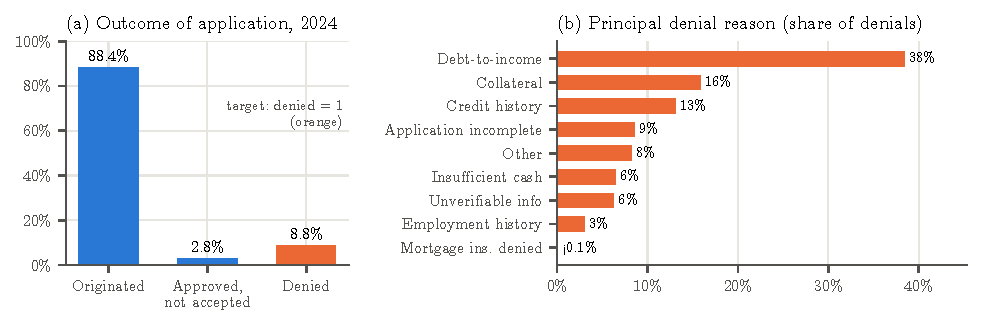
\includegraphics[width=\textwidth]{../../figs/fig1_target.pdf}
\caption{Dependent variable, 2024 ($N=3{,}140{,}857$). (a) Outcome shares. (b) Lender-reported
principal denial reason, used for description and validation only, never as a feature.}
\label{fig:target}
\end{figure}

\subsection{Feature timing and the leakage audit}\label{sec:leak}
Every column is placed in one of three tiers:
\begin{itemize}
  \item \textbf{A} --- known when the application is filed;
  \item \textbf{U} --- produced during underwriting: DTI, combined LTV and property value
  (after the appraisal), the AUS that was run, and the credit-score model (after the credit
  pull);
  \item \textbf{P} --- recorded only after or because of the decision: rate, spread, costs,
  lender credits, HOEPA status, purchaser type, denial reasons, and the pre-approval and
  ``initially payable'' artefacts found in the first submission.
\end{itemize}
Tier~P is never used. Tier~U is used only in model~B.

Within tier U the important question is what a \emph{missing} or ``not applicable'' value
means. Table~\ref{tab:miss} shows that such values pile up in files denied for credit
history or incompleteness. These files are typically rejected before the AUS run or the
appraisal. Four findings follow.
\begin{itemize}
  \item \textbf{AUS.} Among the 394 lenders that run an AUS on more than 98\pct\ of approved
  loans (57\pct\ of all applications), the AUS = ``not applicable'' code appears on 0.7\pct\
  of approved files but on 10.7\pct\ of denied ones. The denial rate when it appears is
  55\pct, against 7\pct\ otherwise. The code records an early rejection, so the AUS field is
  dropped.
  \item \textbf{LTV.} LTV above 100\pct\ is 2.5 times as common among denied conventional
  applications as among approved ones. Of the 10{,}838 applications with LTV above 105\pct,
  56\pct\ are denied, and two thirds of those cite collateral. This is the pattern an
  appraisal coming in below the purchase price would produce, which is why LTV is tier U.
  \item \textbf{DTI and loan term} are missing far more often in early rejections: 6--10\pct\
  and 5.2\pct\ of credit-history denials, against 0.6\pct\ and 0.1\pct\ of approved files.
  \item \textbf{Decision.} No missing-value indicators are used for these fields. Missing
  values are filled with training-fold medians or modes inside the pipeline
  (\texttt{Neutraliser}).
\end{itemize}

\begin{table}[!htbp]
\centering\small
\caption{Share of applications (\%) with the field missing or ``not applicable'', by outcome
and principal denial reason, 2024.}
\label{tab:miss}
\begin{tabular}{@{}lrrrrrrr@{}}
\toprule
 & & AUS & No & \multicolumn{4}{c}{Missing} \\
\cmidrule(l){5-8}
 & $N$ & N/A & score & LTV & Prop.\ val. & DTI & Term \\
\midrule
\tabinput ../../results/t_miss_by_reason.tex
\bottomrule
\end{tabular}
\end{table}

\textbf{Imputation must not leave a fingerprint.} Feature importance exposed a subtler leak.
In an earlier version, ``CLTV minus first-lien LTV'' was the second most important feature of
CatBoost model~B. Missing LTV and property value had each been filled with its own median.
That produced impossible pairs, so the derived feature picked out the imputed rows
(AUC \ImpOld\ for spotting them) and brought the missingness signal back. LTV and property value are now imputed
\emph{consistently} with the loan amount, and the imputed value is rounded to a \$10k
mid-point as in the public data. The AUC drops to \ImpNew. That is below what fields that are never imputed reach (0.58 for
income): the imputed rows are a different mix of loans (60\pct\ are VA), so some
separation is expected. All model-B
results in this report use the corrected pipeline.

\textbf{Automated audit.} The \texttt{LeakageAuditor} computes four checks for every column,
on the training data only:
\begin{itemize}
  \item the out-of-fold AUC of the column alone;
  \item whether any large level (at least 1\pct\ of rows) has an almost certain outcome;
  \item how well the missing indicator predicts the outcome;
  \item a within-lender check: whether codes that are rare at a lender come with a much higher
  denial rate than that lender's base rate.
\end{itemize}
The first three checks can trigger \texttt{drop}, which removes the column. Weaker signals,
including the within-lender check, give \texttt{review}: the column is kept and reported for a
human decision.

On the full 2024 sample, the post-decision controls (rate, spread, costs, lender credits,
HOEPA status, purchaser type, denial reasons, pre-approval flag) are all flagged
\texttt{drop}. ``Initially payable'' is flagged \texttt{review}, with a within-lender lift of
22, and was removed by hand. No tier A or U column is dropped. The \texttt{review} flags fall
on AUS, LTV, property value, loan term and DTI. All are explained above.

Table~\ref{tab:sets} shows why this matters. With all fields, a naive model looks perfect:
ROC-AUC 1.000. With the auditor inside the pipeline, all five folds drop the same eight
post-decision columns. Raw missing and ``not applicable'' codes plus AUS add \SetsCBauc\ ROC-AUC
and \SetsCBpr\ PR-AUC over the neutralised version. That gain comes from the process, not from the
applicant, so it is excluded.

\begin{table}[!htbp]
\centering\small
\caption{Effect of questionable features (gradient boosting, raw features, 5-fold CV on 400k
2024 rows, mean (SD)).}
\label{tab:sets}
\begin{tabular}{@{}lrcc@{}}
\toprule
Feature set & Features & ROC-AUC & PR-AUC \\
\midrule
\tabinput ../../results/t_cv.tex
\tabinput ../../results/t_cv_extra.tex
\bottomrule
\end{tabular}
\end{table}

\subsection{Missing values, outliers and categorical variables}
\begin{itemize}
  \item \textbf{Missing values} are rare: at most 3.1\pct\ for every variable used, except the
  ARM teaser period, which is structurally missing for fixed-rate loans (94\pct). Tier~U
  fields are neutralised as described above. For the boosting models, missing tier~A
  numbers stay NaN and the trees learn the direction. For the logistic regression they are
  filled with training medians.
  \item \textbf{Outliers.} The tails contain obvious keying errors: LTV up to $2\times10^{9}$\pct,
  income up to \$7bn, loan-to-income up to 2{,}255. Trees are not affected by monotone
  transformations or extreme values, so the raw values are kept for them. For the
  logistic regression, numeric variables are winsorised at the training 1st and 99th
  percentiles, money amounts are logged, and DTI, LTV, loan-to-income and payment-to-income
  enter through cubic splines.
  \item \textbf{Categorical variables.}
  \begin{itemize}
    \item Low-cardinality codes (loan type, age band, channel, product flags, DTI bins) are
    native categories in boosting and one-hot encoded in the logit.
    \item The three high-cardinality identifiers (2{,}663 lenders, 418 MSAs, 54 states) are
    target-encoded with \emph{cross-fitting}: each row's encoding comes from other folds, so
    a row never sees its own outcome.
    \item CatBoost uses its own ordered target statistics instead.
  \end{itemize}
  \item \textbf{Continuous versions.} DTI is reported in 19 bins, which we also map to a
  numeric scale (bin mid-points) so that ordering can be used.
\end{itemize}
Descriptive statistics for all 43 variables, raw and engineered, are in the Appendix
(Table~\ref{tab:allvars}).

\subsection{Feature engineering and selection}\label{sec:fe}
Features are built inside the pipeline by \texttt{FeatureBuilder}, either row by row or from
training rows only. The groups were motivated by the EDA:
\begin{itemize}
  \item \textbf{Affordability ratios (tier A):} loan/income, income and loan relative to the
  area median income, the payment on the new loan relative to income (annuity at the 2024
  average 30-year rate and the loan term), and the number of applicants. Trees cannot easily
  form ratios on their own.
  \item \textbf{Lender profile (tier A, no target used):} size (log applications), FHA share,
  broker share, and the median loan/income of the lender's applicants.
  \item \textbf{Program limits (tier U):} DTI minus the program's DTI guideline, and LTV
  minus the program's maximum (including financed fees). The EDA showed, for example, that
  USDA files with a DTI of 45--49\pct\ are denied 89--96\pct\ of the time, against about
  5\pct\ for conventional loans.
  \item \textbf{Cash and second liens (tier U):} down payment/income, and CLTV minus the
  first-lien LTV, which signals down-payment-assistance loans (10\pct\ of files).
\end{itemize}
Figure~\ref{fig:eng} shows the denial rate across deciles of six engineered features. The
features were selected by leave-one-group-out ablation (Table~\ref{tab:fe}). Ratios and the
lender profile carry the gain. Program-limit features add almost nothing, because the trees
already find the DTI $\times$ loan-type interaction, but they are kept for interpretation.
Lender $\times$ loan-type and county target encodings added nothing and were removed. The
auditor flags no engineered feature for \texttt{drop}.

\begin{table}[!htbp]
\centering\small
\caption{Feature engineering and selection (gradient boosting, 5-fold CV on 400k 2024 rows).}
\label{tab:fe}
\begin{tabular}{@{}lcccc@{}}
\toprule
 & \multicolumn{2}{c}{Model A} & \multicolumn{2}{c}{Model B} \\
\cmidrule(lr){2-3}\cmidrule(l){4-5}
 & ROC-AUC & PR-AUC & ROC-AUC & PR-AUC \\
\midrule
\tabinput ../../results/t_fe.tex
\bottomrule
\end{tabular}
\end{table}

\begin{figure}[!htbp]
\centering
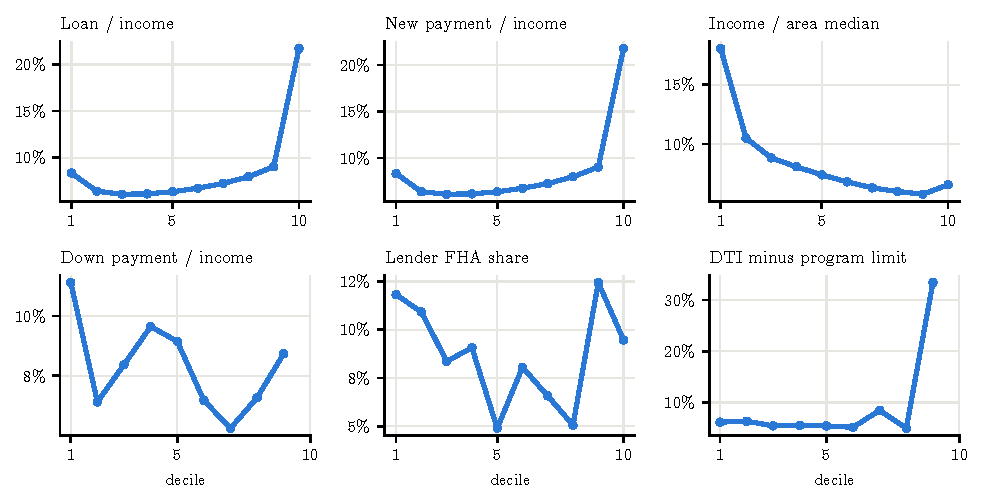
\includegraphics[width=0.92\textwidth]{../../figs/fig6_engineered.pdf}
\caption{Denial rate by decile of six engineered features, 2024.}
\label{fig:eng}
\end{figure}

\textbf{External data.} Three county-level data sets listed on Data.gov were joined by county
FIPS code. Each is lagged so that an application in year $t$ only sees information public at
the time:
\begin{itemize}
  \item FHFA conforming loan limits for year $t$, announced in November of $t-1$; the feature
  is loan/limit for the number of units;
  \item FHFA county house price growth in $t-1$ and over $t-4$ to $t-1$;
  \item BLS county unemployment in $t-1$, and its change from $t-2$.
\end{itemize}
The match rate is 98.7--99.6\pct. These features change the CV metrics by at most 0.001,
which is less than the fold-to-fold noise. Geography is already captured by the MSA and state
encodings and the tract variables. They are kept out of the main specification. Whether
they help the model \emph{transfer} to 2025 is a pre-registered test for the final stage.

%================================================================== 4. METRIC
\section{Performance measure and business goal}\label{sec:metric}
The classes are imbalanced (8.8\pct\ denials), so accuracy is uninformative: approving
everyone is 91\pct\ accurate. The \textbf{primary metric is PR-AUC} (average precision). It
summarises the precision--recall trade-off that matters to users, and its no-skill value is
the denial rate, 0.088. ROC-AUC is reported alongside. The business meaning is clearest as
\emph{precision at a fixed recall}, i.e.\ how many of the flagged files are really denied.
\begin{itemize}
  \item For a \emph{pre-application tool}, a false alarm discourages a borrower who would
  have been approved, and a miss costs the applicant application and appraisal fees plus a
  hard credit inquiry.
  \item For a \emph{lender}, flagged files go to senior underwriters, so precision determines
  how much of their time is wasted.
\end{itemize}
The decision threshold will therefore be chosen from an explicit cost ratio in the final
stage. Calibration (Brier score, log-loss) is monitored because the models output
probabilities that a supervisor would aggregate by lender.

Table~\ref{tab:prec} compares the final model B with the two rule-based screens from the
first submission on the same 300k validation rows.

\begin{table}[!htbp]
\centering\small
\caption{Precision at a given recall on the fixed 2024 validation set (300k rows).
``Flagged'' is the share of all applications that are flagged.}
\label{tab:prec}
\begin{tabular}{@{}lccc@{}}
\toprule
Screen & Recall & Precision & Flagged \\
\midrule
\tabinput ../../results/t_prec.tex
\bottomrule
\end{tabular}
\end{table}

%======================================================== 5. MODELS / RESULTS
\section{Learning algorithms and preliminary cross-validated results}
\begin{itemize}
  \item \textbf{Logistic regression} with an L2 penalty is the interpretable benchmark, with
  the design described above. The penalty $C\in\{0.01,0.1,1\}$ is chosen by CV.
  \item \textbf{Histogram gradient boosting} (scikit-learn), with hyper-parameters tuned by
  successive halving: 16 random configurations, the better half moving on to twice as many
  rows, from 50k to 400k, with 3-fold CV and PR-AUC as the criterion.
  \item \textbf{CatBoost}, which handles categorical variables natively. Eight random
  configurations were tried on a separate 100k/100k train / early-stopping split. All eight
  landed within 0.008 PR-AUC of each other. We took the fastest configuration within 0.002
  of the best, which turned out to be the default settings (depth 8, learning rate 0.1). The
  final models are trained on all 2.74m training rows (8-core Apple M3, 16\,GB; about 2 hours
  for model B and 1.2 hours for model A). They stop early on a separate 100k set, with a cap of
  4{,}000 trees that was never reached: model A stopped at \FinAiter\ trees and model B at
  \FinBiter.
\end{itemize}
All learners share the same leakage-safe pipeline:
\texttt{Neutraliser} $\rightarrow$ \texttt{FeatureBuilder} $\rightarrow$ encoding $\rightarrow$
model. It is fitted inside every training fold.

\begin{table}[!htbp]
\centering\small
\caption{Preliminary results. Top: 5-fold CV on the same 400k 2024 rows. Bottom: models trained
on large 2024 training sets (gradient boosting: all 2.84m pool rows; CatBoost: all 2.74m training rows), evaluated on the fixed 300k validation set.}
\label{tab:models}
\begin{tabular}{@{}lcccc@{}}
\toprule
 & \multicolumn{2}{c}{Model A (application time)} & \multicolumn{2}{c}{Model B (+ underwriting)} \\
\cmidrule(lr){2-3}\cmidrule(l){4-5}
 & ROC-AUC & PR-AUC & ROC-AUC & PR-AUC \\
\midrule
\tabinput ../../results/t_models.tex
\midrule
\tabinput ../../results/t_models_full.tex
\bottomrule
\end{tabular}
\end{table}

Four results stand out (Table~\ref{tab:models}, Figure~\ref{fig:lc}).
\begin{itemize}
  \item \textbf{Flexible learners clearly beat the logit.} The gap is largest in model B
  (PR-AUC \LogitBpr\ vs \CatBpr), where denials depend on non-linear combinations such as DTI
  relative to the program's limit.
  \item \textbf{Engineered features add more than tuning.} Feature engineering adds \FEgainA\ PR-AUC to
  model A and \FEgainB\ to model B. Tuning the boosting model adds \TuneGainA\ and \TuneGainB.
  \item \textbf{CatBoost is the strongest learner.} It beats tuned gradient boosting by two to
  three times the fold-to-fold standard deviation. Its handling of lender and geography
  identifiers is the likely reason.
  \item \textbf{More data keeps helping.} Performance has not levelled off at 2.84 million
  rows. The final CatBoost models are therefore trained on all 2.74 million
  training rows. They reach ROC-AUC \FinBauc\ / PR-AUC \FinBpr\ (model B) and
  \FinAauc\ / \FinApr\ (model A) on the fixed validation set.
  They are well calibrated: mean predicted probability \FinBmean\ against an observed rate of
  \FinBbase, Brier score \FinBbrier.
\end{itemize}

\begin{figure}[!htbp]
\centering
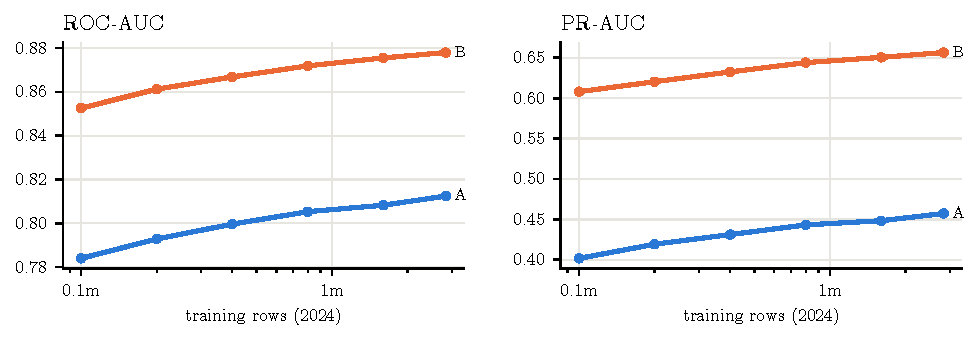
\includegraphics[width=0.92\textwidth]{../../figs/fig5_learning_curve.pdf}
\caption{Learning curve: gradient boosting trained on 100k to 2.84m 2024 rows, evaluated on the
fixed 300k validation set.}
\label{fig:lc}
\end{figure}

%============================================================== 6. FINAL PLAN
\section{Plan for the final stage}
The tests below are fixed now, before the hold-out is opened.
\begin{enumerate}
  \item \textbf{Validation on 2025.} One-time evaluation of the final models A and B. We
  report ROC-AUC, PR-AUC, precision at 30/50/70\pct\ recall, calibration, and the change from
  2024, with bootstrap confidence intervals.
  \item \textbf{Temporal robustness.} Models with and without the external county data are
  compared on 2025, together with monotonic constraints on DTI, LTV and payment-to-income.
  \item \textbf{Interpretation.} Feature importance, partial dependence and SHAP values. SHAP
  explanations will be compared with the denial reasons that lenders report.
  \item \textbf{Fairness audit.} Calibration and the gap in denial rates by race and
  ethnicity that remains after conditioning on the model's prediction, with and without
  neighbourhood variables that may act as proxies.
  \item \textbf{Economic value.} Expected savings in fees and underwriting time for the chosen
  threshold.
\end{enumerate}

\vspace{2pt}
\textbf{Code and data.} All code is submitted. It covers sample construction, the
feature-timing diagnostics, the leakage auditor, feature engineering, external data,
cross-validation, tuning and final training. A README gives the run order. The analysis
samples (parquet, $\approx$75\,MB per year) and the external county table are included. The
raw HMDA files ($\approx$3.3\,GB) are downloaded by the code.

\vspace{-4pt}
\begin{thebibliography}{9}\footnotesize
\setlength{\itemsep}{-1pt}
\bibitem{fuster2022} Fuster, A., Goldsmith-Pinkham, P., Ramadorai, T., Walther, A. (2022).
Predictably unequal? The effects of machine learning on credit markets. \emph{Journal of
Finance}, 77(1), 5--47.
\bibitem{islp} James, G., Witten, D., Hastie, T., Tibshirani, R., Taylor, J. (2023).
\emph{An Introduction to Statistical Learning with Applications in Python}. Springer.
\bibitem{catboost} Prokhorenkova, L., Gusev, G., Vorobev, A., Dorogush, A., Gulin, A. (2018).
CatBoost: unbiased boosting with categorical features. \emph{NeurIPS} 31.
\bibitem{halving} Jamieson, K., Talwalkar, A. (2016). Non-stochastic best arm identification
and hyperparameter optimization. \emph{AISTATS}.
\bibitem{cfpb} CFPB/FFIEC. HMDA Data Browser and Filing Instructions Guide (2024, 2025).
\url{https://ffiec.cfpb.gov/}.
\bibitem{fhfa} FHFA. Conforming Loan Limit Values; House Price Index, county annual. Listed on
Data.gov. \url{https://www.fhfa.gov/data}.
\bibitem{bls} BLS. Local Area Unemployment Statistics, county annual averages. Listed on Data.gov.
\url{https://www.bls.gov/lau/}.
\end{thebibliography}

%=================================================================== APPENDIX
\clearpage
\appendix
\section*{Appendix: descriptive statistics of all variables (2024, $N=3{,}140{,}857$)}
Tier A = application time, U = underwriting time, FE = engineered. For numeric variables:
P1 / median / P99. For categorical variables: number of levels and share of the most common
level. Engineered features are computed after neutralisation, so they have no
underwriting-time missing values.

\begin{table}[!htbp]
\centering\footnotesize
\caption{All variables used by models A and B.}
\label{tab:allvars}
\begin{tabular}{@{}llllp{5.2cm}@{}}
\toprule
Variable & Tier & Type & Miss.\,\% & Distribution \\
\midrule
\tabinput ../../results/t_all_vars.tex
\bottomrule
\end{tabular}
\end{table}

\begin{figure}[!htbp]
\centering
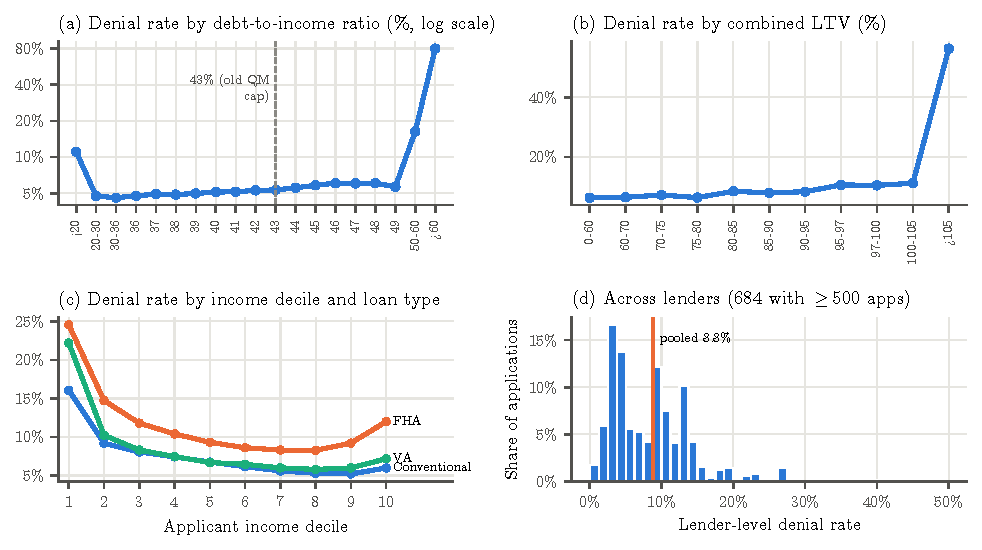
\includegraphics[width=\textwidth]{../../figs/fig2_predictors.pdf}
\caption{Denial rate against the main raw predictors, 2024 (from the first submission): (a) DTI,
(b) combined LTV, (c) income decile by loan type, (d) lender-level denial rates.}
\end{figure}

\end{document}
